% !Rnw weave = knitr
\documentclass[12pt]{article}\usepackage[]{graphicx}\usepackage[]{color}
% maxwidth is the original width if it is less than linewidth
% otherwise use linewidth (to make sure the graphics do not exceed the margin)
\makeatletter
\def\maxwidth{ %
  \ifdim\Gin@nat@width>\linewidth
    \linewidth
  \else
    \Gin@nat@width
  \fi
}
\makeatother

\definecolor{fgcolor}{rgb}{0.345, 0.345, 0.345}
\newcommand{\hlnum}[1]{\textcolor[rgb]{0.686,0.059,0.569}{#1}}%
\newcommand{\hlstr}[1]{\textcolor[rgb]{0.192,0.494,0.8}{#1}}%
\newcommand{\hlcom}[1]{\textcolor[rgb]{0.678,0.584,0.686}{\textit{#1}}}%
\newcommand{\hlopt}[1]{\textcolor[rgb]{0,0,0}{#1}}%
\newcommand{\hlstd}[1]{\textcolor[rgb]{0.345,0.345,0.345}{#1}}%
\newcommand{\hlkwa}[1]{\textcolor[rgb]{0.161,0.373,0.58}{\textbf{#1}}}%
\newcommand{\hlkwb}[1]{\textcolor[rgb]{0.69,0.353,0.396}{#1}}%
\newcommand{\hlkwc}[1]{\textcolor[rgb]{0.333,0.667,0.333}{#1}}%
\newcommand{\hlkwd}[1]{\textcolor[rgb]{0.737,0.353,0.396}{\textbf{#1}}}%
\let\hlipl\hlkwb

\usepackage{framed}
\makeatletter
\newenvironment{kframe}{%
 \def\at@end@of@kframe{}%
 \ifinner\ifhmode%
  \def\at@end@of@kframe{\end{minipage}}%
  \begin{minipage}{\columnwidth}%
 \fi\fi%
 \def\FrameCommand##1{\hskip\@totalleftmargin \hskip-\fboxsep
 \colorbox{shadecolor}{##1}\hskip-\fboxsep
     % There is no \\@totalrightmargin, so:
     \hskip-\linewidth \hskip-\@totalleftmargin \hskip\columnwidth}%
 \MakeFramed {\advance\hsize-\width
   \@totalleftmargin\z@ \linewidth\hsize
   \@setminipage}}%
 {\par\unskip\endMakeFramed%
 \at@end@of@kframe}
\makeatother

\definecolor{shadecolor}{rgb}{.97, .97, .97}
\definecolor{messagecolor}{rgb}{0, 0, 0}
\definecolor{warningcolor}{rgb}{1, 0, 1}
\definecolor{errorcolor}{rgb}{1, 0, 0}
\newenvironment{knitrout}{}{} % an empty environment to be redefined in TeX

\usepackage{alltt}
\usepackage[backend=biber, sorting=nyt, maxcitenames=2, doi=false,url=false, style=apa]{biblatex} 
\bibliography{/home/harold/Dropbox/full,/home/harold/github/eysterthesis/manuscript/thesis_ref}
\DeclareLanguageMapping{american}{american-apa}
\usepackage{xr}
\externaldocument{Eyster_germ_ms}
\renewcommand{\thetable}{S\arabic{table}} 
\renewcommand{\thefigure}{S\arabic{figure}}
\usepackage{graphicx}
\graphicspath{}
\usepackage{caption}
\usepackage{subcaption}
\captionsetup[subfigure]{position=top}
\usepackage[figuresleft]{rotating}
\usepackage{longtable}
\usepackage[margin=1in]{geometry}
\usepackage{float}
\usepackage{makecell}
\usepackage{amsmath}
\usepackage{mathtools}
\usepackage{breqn}
\usepackage{url}
\usepackage{afterpage}
%R -e "knitr::knit2pdf('SI.rnw')" 


\title{\textbf{Supporting information for:}  \\ \bigskip Comparisons in the native and introduced ranges reveal little evidence of climatic adaptation in germination traits}\author{Harold N. Eyster* \&  Elizabeth Wolkovich}
\date{*Corresponding author. Please direct any questions or comments to haroldeyster@gmail.com. }





\IfFileExists{upquote.sty}{\usepackage{upquote}}{}
\begin{document}
\maketitle
\tableofcontents
\section{Additional general methods}
\subsection{Defining Invasive Species}
There is no consensus on how to classify a species as invasive \parencite{Colautti2004}. The most common terms include `exotic,' `introduced,' `naturalized,' `nonindigenous,' `established,' `alien,' `noxious,' `weedy,' and `invasive.' These terms can be grouped into those that describe the provenance of the species (e.g., exotic, introduced, alien, non-indigenous), those that describe its ability to grow and compete in the new ecosystem (e.g., naturalized, established), and those that describe its impact on the receiving ecosystem (e.g., noxious, weedy, harmful). The International Union for the Conservation of Nature (IUCN, 2008) describes invasive species as: ``organisms introduced by man [sic] into places out of their natural range of distribution, where they become established and disperse, generating a negative impact." \nocite{IUCN2008is} However, this definition contains three subjective elements: what timepoint of a species' range is `natural,' whether humans are a natural part of nature, and what is defined as a negative impact \parencite{Munro2019}. To both acknowledge and allay some of these subjective elements, this paper follows the definition of \textcite{Richardson2000,Richardson2011}. Invasive species are thus those that (1) are introduced across a previously unpenetrated barrier, (2) successfully reproduce in the place of introduction to create a stable local population, and finally (3) spread to produce fit offspring a substantial distance from the place of introduction.

\subsection{Study species details}
\textit{Capsella bursa-pastoris} (CAPBUR; Shepard's Purse) is an annual or biennial herbaceous plant in Brassicaceae. It grows 10 to 80 cm tall, typically blooming in late spring \parencite{Defelice2001}. It originated in Europe, and was introduced to the New World as a medicinal herb---it is now found across Canada, the US, and Mexico \parencite{Westrich1989}.
	
	\textit{Chelidonium majus} (CHEMAJ; Greater Celandine) is an herbaceous biennial member of Papaveraceae. It is native to Europe, Asia, and North Africa and was introduced to the US by the 1670s as a medicinal. It is now found across the Eastern US and Canada and portions of the west \parencite{Holm1979}. 
	
	\textit{Dactylis glomerata} (DACGLO; Orchard Grass) is a cool-season, perennial grass (Poaceae). Plants grow up to 120 cm tall and have roots up to 60 cm long \parencite{Moser1996}. This plant originated in  Europe, Asia, and North Africa, and was intentionally introduced into the US in the 1750s \parencite{Bush2012} as a forage grass for pasture and hay \parencite{Ogle2011}.  It is now found across North America, stretching from Atlantic Canada to the Pacific coast.
	
	\textit{Plantago lanceolata} (PLALAN; Narrow-leaved Plantain) is a perennial member of  Plantaginaceae. It has narrow, ribbed leaves and grows to 1 m tall. It is native to Eurasia, and has successfully colonized the world's mid-latitudes \parencite{Holm1977}.
	
	\textit{Plantago major} (PLAMAJ; Broad-leaved Plantain) is a perennial member of Plantaginaceae. It has broad, smooth leaves, and grows to 15 cm tall. Native to Europe and Asia,  it was introduced into North America for its medicinal uses, and now is found across North America, from Florida to Alaska \parencite{Knobloch1996,Samuelsen2000}.
	
	\textit{Rumex crispus} (RUMCRI; Curly Dock) is a perennial herbaceous plant in Polygonaceae, and grows to 160 cm. It is native to Europe, Asia, and Africa, and was introduced for its medicinal uses into North America where it now found across much of the continent \parencite{USDA2010}. 
	
	\textit{Taraxacum officinale} (TAROFF; Dandelion) is a perennial herbaceous plant in Asteraceae, and grows to 60 cm. It is native to Eurasia, but is now found in all 50 US states, much of Canada, and Mexico \parencite{USDA1971}.

\subsection{Sampling details}
Numbers of sampled populations and individual plants from which we collected seeds are given in Table \ref{tab:seednum}. We used Bayesian multilevel models to account and control for   greater sampling in the source range. % Additionally, we note that our results go in the opposite direction of this sampling bias---given the limited number of sampled populations in the introduced range we were more likely to find differences between the native and introduced ranges. 
	\begin{center}
		\begin{table}[H]
			\centering
			\caption {Total number of seed-producing individuals and populations from which seeds were collected.} \label{tab:seeds}  
			\begin{tabular}{c|c|c|c}
				\makecell{\textbf{US} \\ \textbf{populations}} & \makecell{\textbf{US} \\  \textbf{individuals}} & \makecell{\textbf{European} \\ \textbf{populations}} & \makecell{\textbf{European} \\ \textbf{individuals}} \\
				\hline
				3&	21&	13&	63\\
			\end{tabular}
			\label{tab:seednum}
		\end{table}
	\end{center}
	
\subsection{Selecting period/light luminance}
Some species have sufficient Pfr (the active form of phytochrome pigment, often necessary to induce germination) and so do not need any light to break dormancy, others just need a pulse of red light to break dormancy \parencite[the red light converts the inactive phytochrome into Pfr,][]{Casal998}.  Other species, including \textit{Plantago major}, take much longer to build up the requisite Pfr, and so have much higher germination success when exposed to longer periods of light \parencite[with nearly 100\% germination after 48 hours of exposure for \textit{P. major},][]{Pons1991}. Finally, some species have a high irradiance response (HIR), germinating poorly when exposed to high luminance light or prolonged light \parencite{Roberts1987}. Beyond interspecific variation, there is also intraspecific variation in the relationship between dormancy and light \parencite{Probert1986}. Across all populations, germination success seems to be log-normally related to photon dosage \parencite{Ellis1986}. Light may begin inhibiting germination for HIR species at about 0.1 mol/m\textsuperscript{2}/day--1 mol/m\textsuperscript{2}/day \parencite{Baskin1998,Ellis1986}, while other species peak above 10 mol/m\textsuperscript{2}/day \parencite{Ellis1986}. The differing levels of light necessary to break dormancy means that any chosen light regime will be better for some species and worse for others. 
	
	The goal of these experiments was to create germination levels that are sufficient to observe variation in responses to treatments. Thus, we chose an intermediate light exposure at which all of the species would germinate at substantial levels, but which may not be ideal for any species. In selecting how much light to use, this experiment erred on the side of too much light rather than not enough, since at least one of our species is known to need large amounts of light \parencite[\textit{Plantago major},][]{Pons1991}, but none are known to exhibit HIR \parencite[although a \textit{D. glomerata} subspecies in southern Europe does exhibit HIR, see][however, this subspecies is not thought to have been collected for this study]{Probert1986}. Thus this experiment used a length of eight hours at a luminance of 75 micromol/m\textsuperscript{2}/second to yield a daily photon dosage of 2.16 mol/m\textsuperscript{2}. \textcite{Baskin1998} recommend that the light period coincide with the high-temperature period. Thus, this experiment exposed seeds to eight hours of fluorescent light during the high-temperature thermoperiod. 
	
\subsection{Selecting substrate and planting depth} 
Substrate and planting depth can affect germination. \textcite{Popay1970} show that \textit{C. bursa-pastoris} seeds germinated about equally on filter paper as on top of soil, but showed much decreased germination when inserted into soil. However, the effects of planting substrate and depth have not been studied in most of the study species. Nevertheless, a study on a species related to \textit{D. glomerata} suggests that \textit{D. glomerata} may germinate better in soil \parencite{Andrews1974}. Moreover, a difference in depth of just a couple millimeters can result in extreme differences in light availability, which can be essential for germination \parencite{Tester1987}. Thus each seed was placed on top of Fafard Growing Mix (a mixture of fine peat moss, fine perlite, and vermiculite) soil, with each seed in its own individual tray cell.

\subsection{Average predictive comparisons} 
Average Predictive Comparisons can increase the interpretability of variables in complex (e.g., multilevel and interactive) models \parencite{Gelman2007}.  The average predictive comparison for an input variable, $\upsilon$, is: 

\begin{align}
APC = \widehat{\Delta} \upsilon =  \left( \frac{\sum_{i=1}^{n} \sum_{k=1}^{K} \sum_{s=1}^{S} [\sum_{j\space \epsilon(k)} \omega(\upsilon_i,\upsilon_j)]E(y|\upsilon^{k}, \nu_i,\theta^s) - E(y|\upsilon_i, \nu_i,\theta^s)} {S \sum_{i=1}^{n} \sum_{k=1}^{K}[\sum_{j\space \epsilon(k)} \omega(\upsilon_i,\upsilon_j)]} \right) ^{\frac{1}{2}}
\end{align}
Where $n$ is the number of observations in the data, $\theta$ is the model with $s$ independent sets of parameter draws (Bayesian iterations), $y$ is the response variable, $\upsilon$ is the input variable of interest with $k$ levels, and $\nu$ is a vector of all the other variables (i.e., all the variables except $\upsilon$). 
Average predictive comparisons are distinct from partial derivatives, since APCs do not collapse $\upsilon^{2} - \upsilon^{1}$ to zero, but retain the unit differences found in the data. 

Because our study uses a balanced, full factorial design, we can ignore the weighting function, $\omega(\upsilon_i,\upsilon_j)$, which is the likelihood that $\upsilon$ transitions from $\upsilon_i$ to $\upsilon_j$ when $\nu = \nu_i$. 

We also calculated the standard error of the average predictive comparison according to: 

\begin{align}
S.E.(\widehat{\Delta_\upsilon})=\frac{1}{2 \widehat{\Delta_\upsilon}}\left( \frac{1}{S-1} \sum_{s=1}^S[(\widehat{\Delta_\upsilon^s})^2-(\widehat{\Delta_\upsilon})^2]^{2} \right)^{\frac{1}{2}}
\end{align}

For a worked example see: \url{http://htmlpreview.github.io/?https://github.com/hneyster/germination_stan/blob/master/APC.html}.


Average predictive comparisons complement model results to better interpret our findings. For example, in Figure \ref{fig:apc} (main text),
the estimates for germination success are due to inconsistent,
idiosyncratic effects that are not generalizable but appear because of a
combination of the APC method and these particular results: APCs take
the sum of squared differences (see equation above) and shows that seeds stratified at 60 days rather
than 30 days had plus or minus 43\% probability of germinating (i.e.,
they were either more likely or less likely to germinate---the model
results in Figure \ref{fig:coef} show that these positive and negative differences are just random and
balance each other out).
\printbibliography

\section{Unmodeled Data Plots}
Below we provide plots of the unmodeled data. In the main text we show model estimates because they provide best estimates that account for much of the variance and pseudoreplication in the data (as the model integrates over seed family, population, and species). % However, these effects may be obscured in the aggregate raw data plots shown here.
\begin{figure}[H]
  \centering
  \subcaptionbox{CAPBUR\label{fig:grCAPBUR}}
  {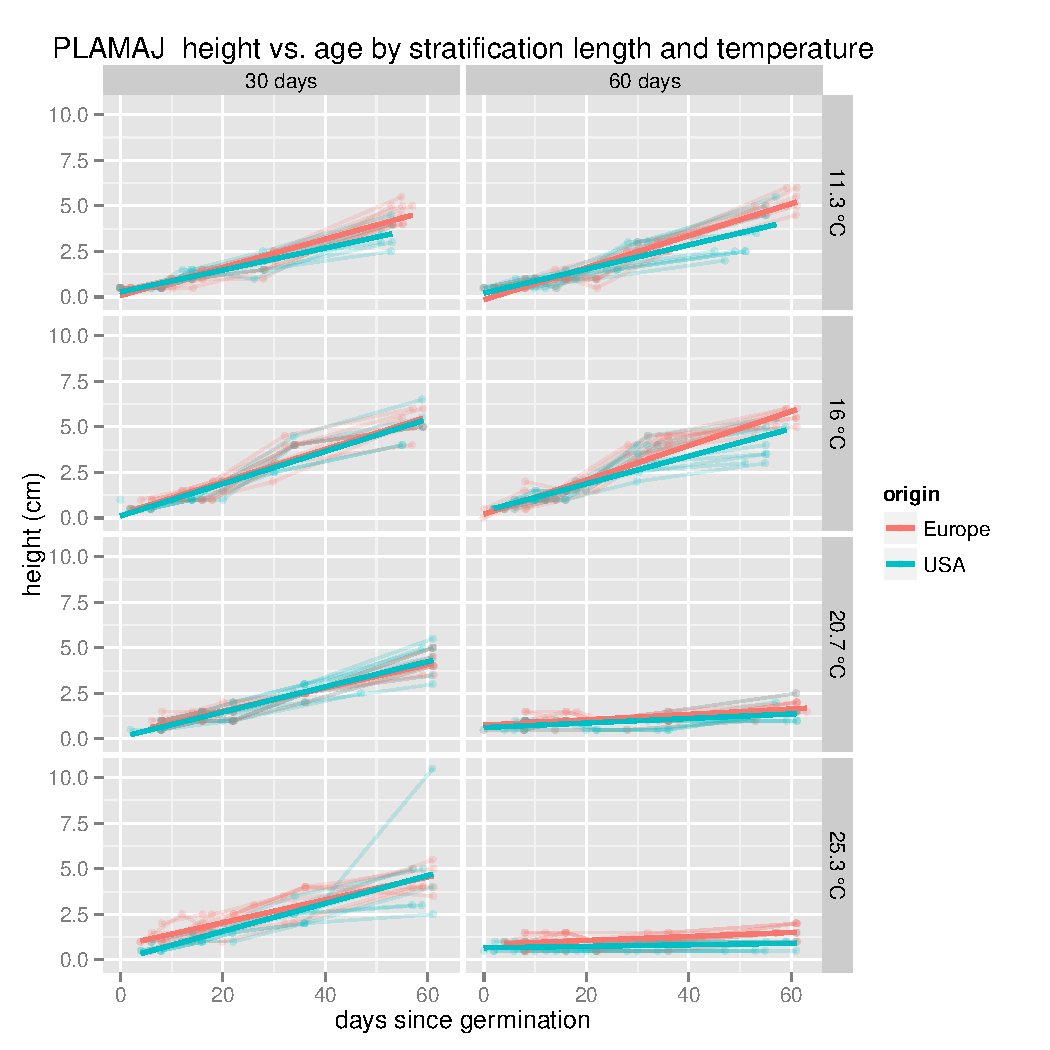
\includegraphics[scale=.5, page=1, trim=0cm 0cm 2.9cm 0cm, clip=TRUE]{supplement.pdf}}
  \subcaptionbox{CHEMAJ\label{fig:grCHEMAJ}}
  {\includegraphics[scale=.5, page=2, trim=0cm 0cm 2.9cm 0cm, clip=TRUE]{supplement.pdf}}
  \subcaptionbox{DACGLO\label{fig:grDACGLO}}
  {\includegraphics[scale=.5, page=3, trim=0cm 0cm 2.9cm 0cm, clip=TRUE]{supplement.pdf}}
  \subcaptionbox{PLALAN\label{fig:grPLALAN}}
  {\includegraphics[scale=.5, page=4, trim=0cm 0cm 2.9cm 0cm, clip=TRUE]{supplement.pdf}}
\end{figure}
\begin{figure}[H]\ContinuedFloat
  \centering
  \subcaptionbox{PLAMAJ\label{fig:grPLAMAJ}}
  {\includegraphics[scale=.5, page=5, trim=0cm 0cm 2.9cm 0cm, clip=TRUE]{supplement.pdf}}
  \subcaptionbox{RUMCRI\label{fig:grRUMCRI}}
  {\includegraphics[scale=.5, page=6, trim=0cm 0cm 2.9cm 0cm, clip=TRUE]{supplement.pdf}}
  \subcaptionbox{TAROFF\label{fig:grTAROFF}}
  {\includegraphics[scale=.5, page=7, trim=0cm 0cm 0cm 0cm, clip=TRUE]{supplement.pdf}}
  \caption{Height vs. age by stratification and temperature, which shows that growth rate was approximately linear.  Pink represents European plants, while blue represents those from  North America.}\label{fig:lmgr}
\end{figure}
\afterpage{%
	\thispagestyle{empty}
\begin{figure}[H]
  \centering
  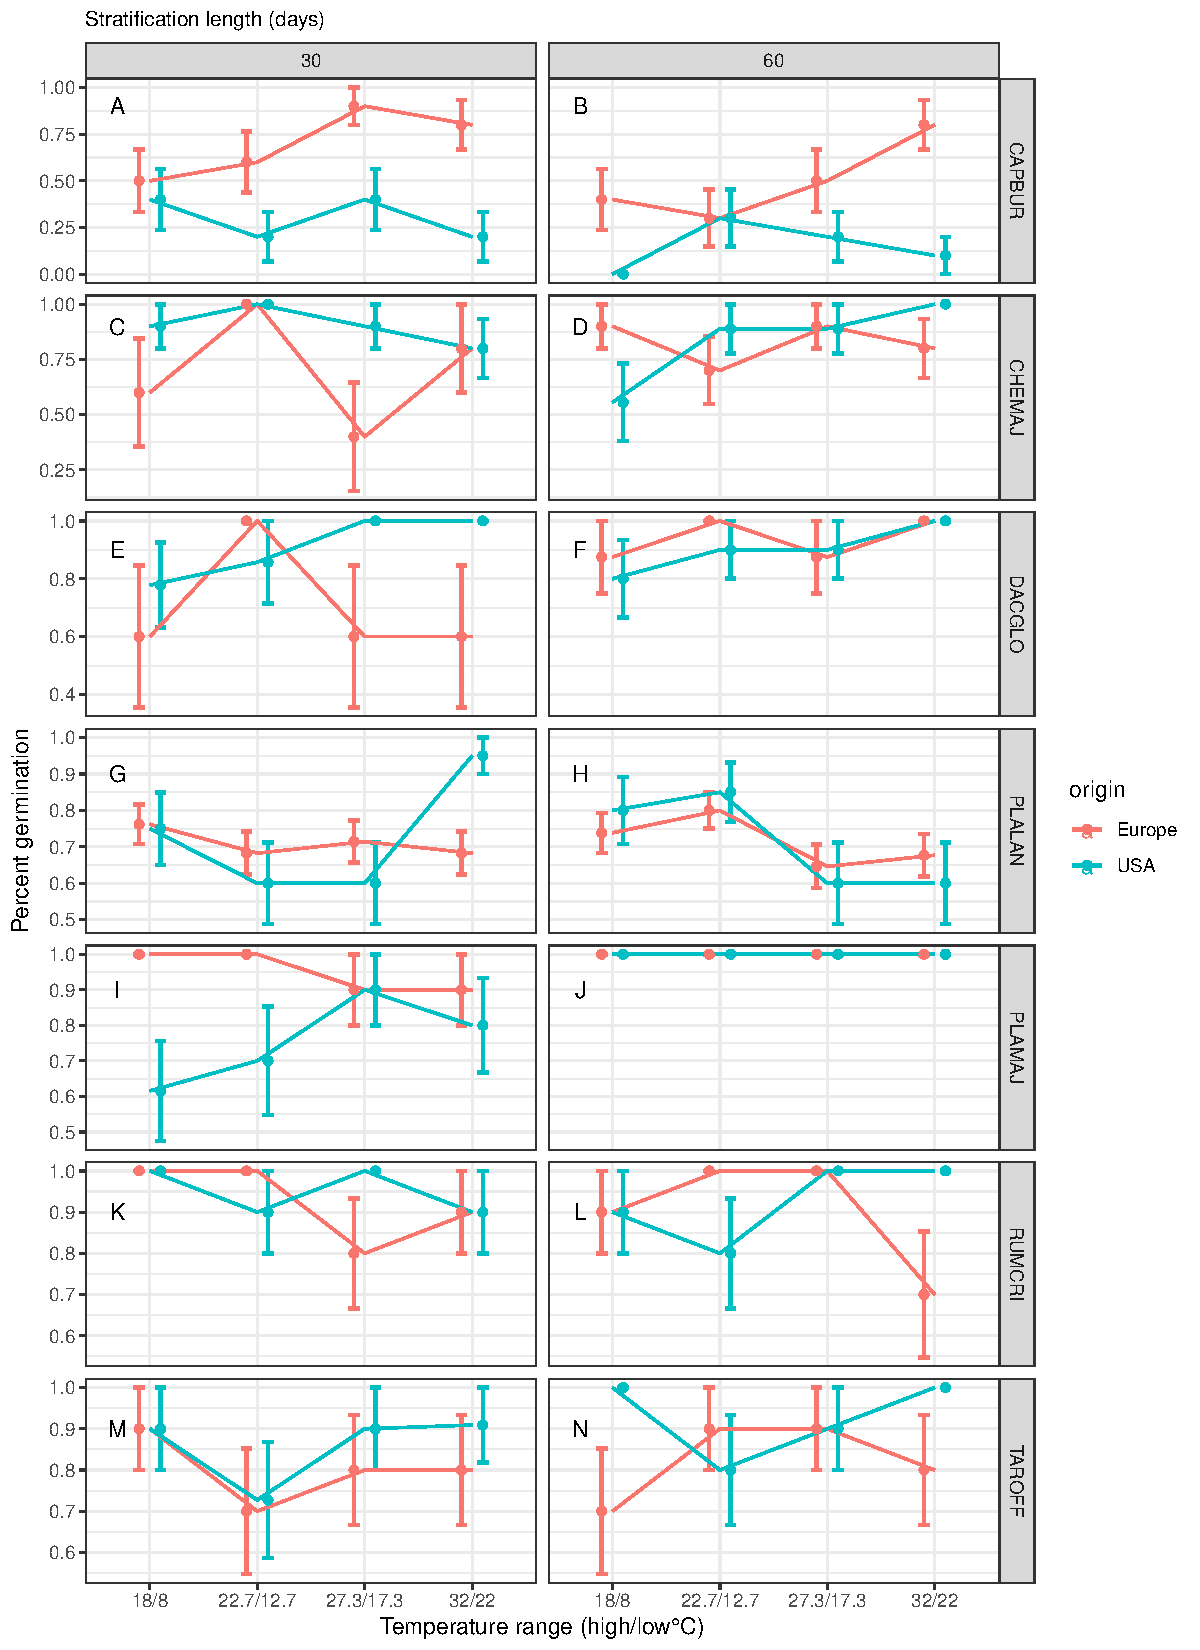
\includegraphics[scale=.8]{figure5}  %EMWAug19: maybe try scale of 0.8 or lower so the caption shows up?
  \caption{Unmodeled germination success by population origin, and across stratification length and temperature treatments for each species (mean +/- standard error). Note the variable y-axis scale. Significant modeled parameters are indicated (based on 95\% credible intervals. The modeled reference level for temperature is a high of 18$^\circ$C, Sixty days is the reference level for stratification, and Europe is the reference level for population origin.} \label{fig:rawrate}
\end{figure}
}
\afterpage{%
	\thispagestyle{empty}
\begin{figure}[H]
  \centering
  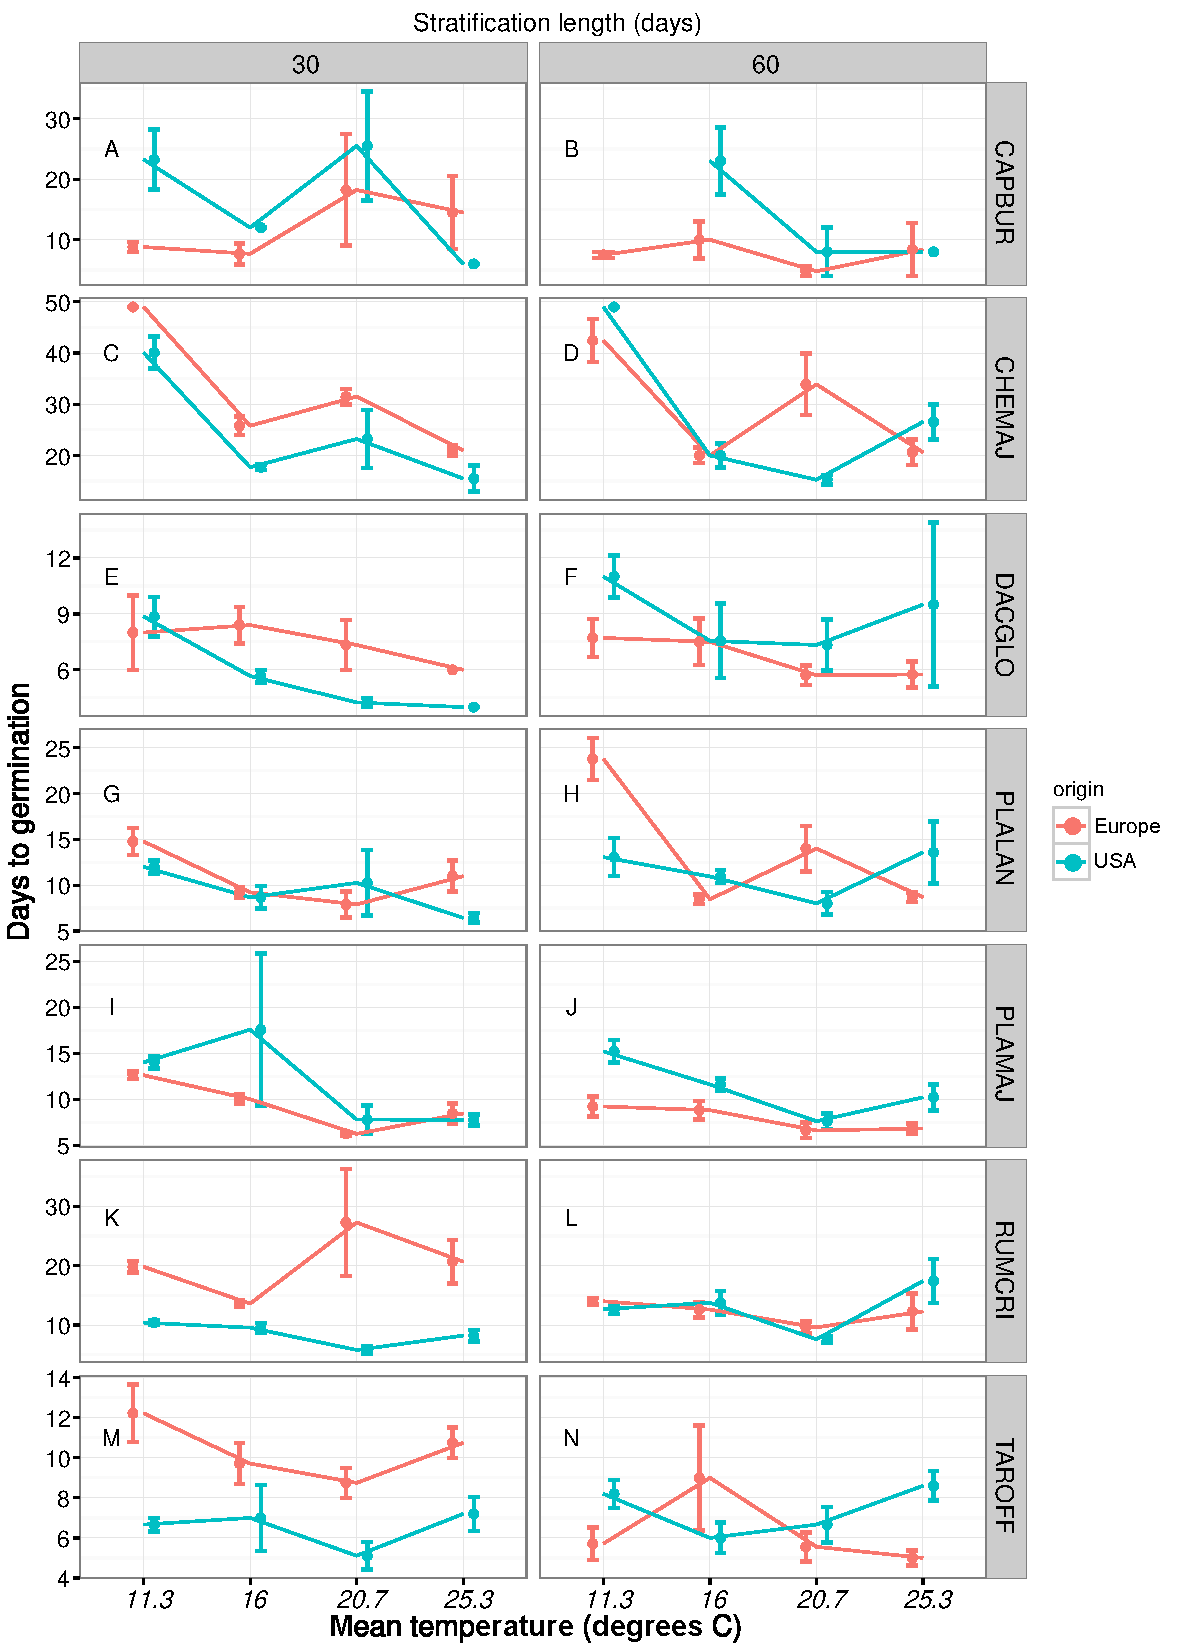
\includegraphics[scale=.8]{figure7} %EMWAug19: maybe try scale of 0.8 or lower so the caption shows up?
  \caption{Unmodeled germination timing by population origin, and across stratification length and temperature treatments for   each species (mean +/- standard error). Note the variable y-axis scale. Significant model results are indicated (based on 95\% credible intervals). The modeled reference level for temperature is a high of 18$^\circ$C, Sixty days is the reference level for stratification, and Europe is the reference level for population origin.} \label{fig:rawtime} 
\end{figure}
}
\afterpage{%
	\thispagestyle{empty}
\begin{figure}[H]
  \centering
  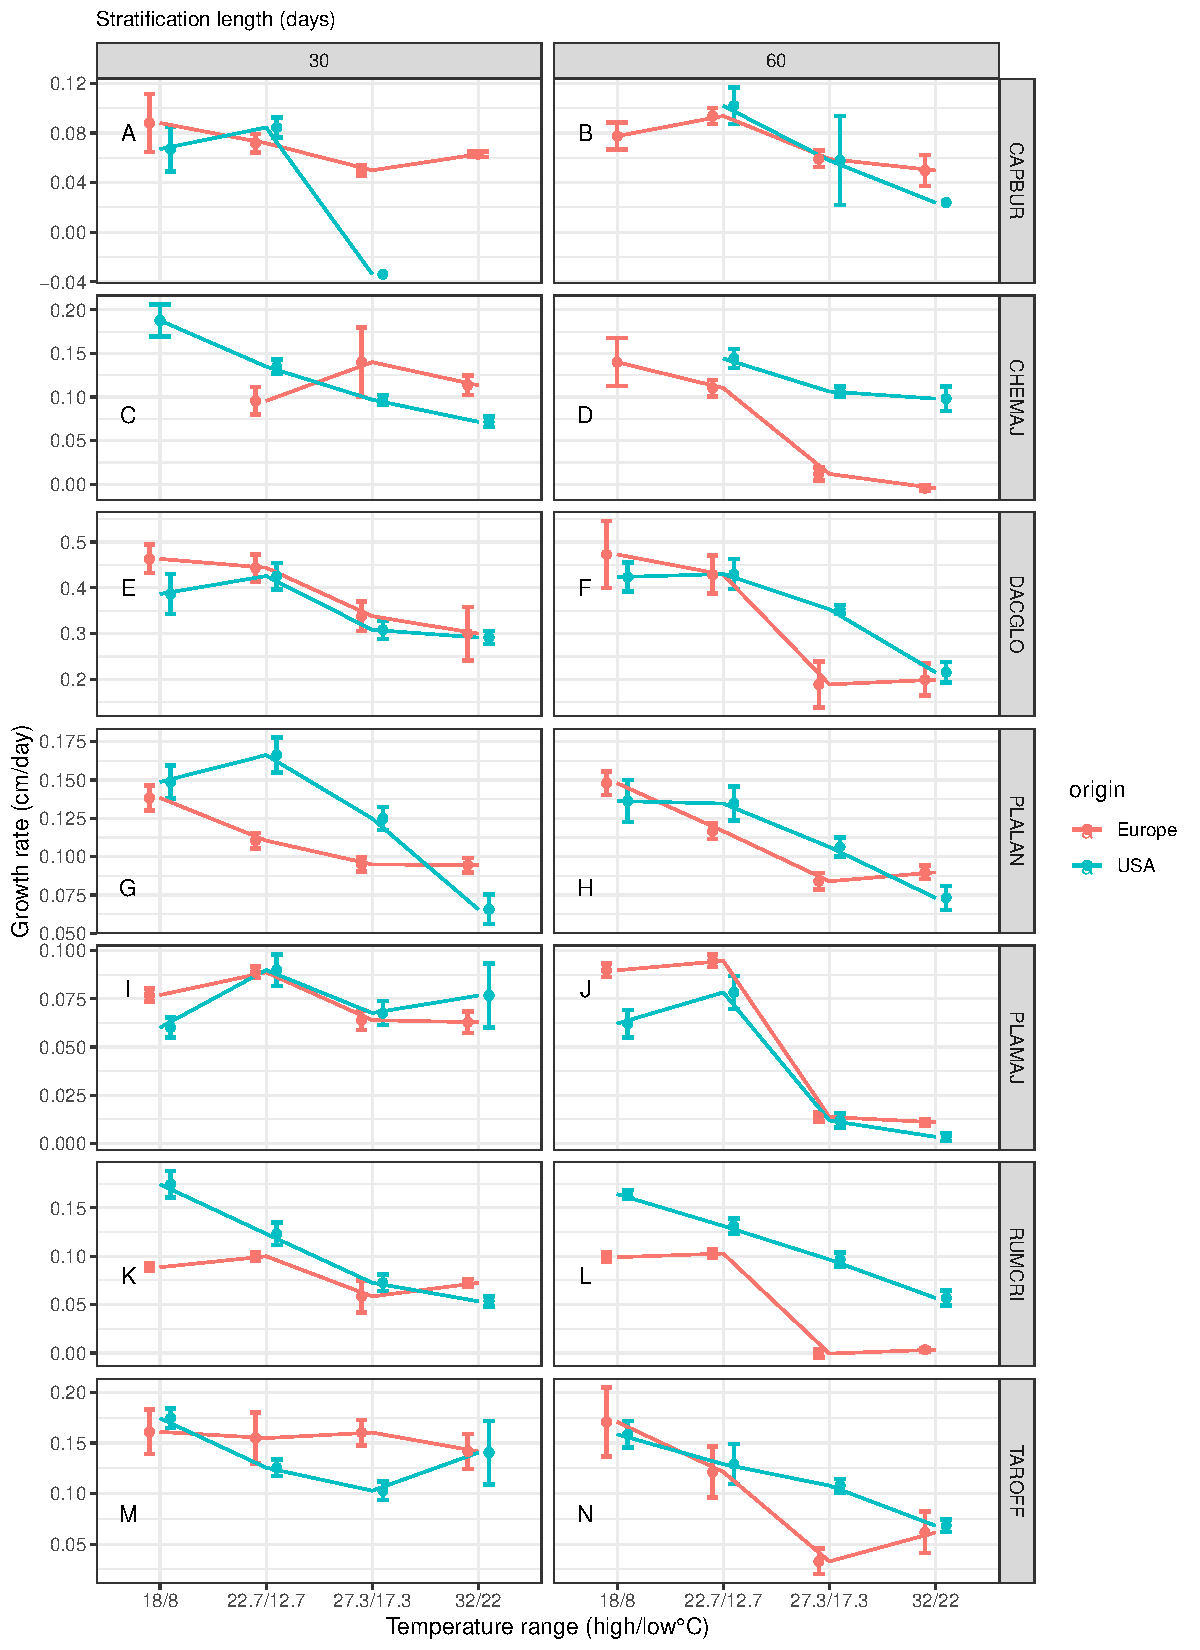
\includegraphics[scale=.8]{figure9} %EMWAug19: maybe try scale of 0.8 or lower so the caption shows up?
  \caption{Unmodeled growth rate by population origin, and across stratification length and temperature treatments for each   species (mean +/- standard error). Note the variable y-axis scale. Significant model results are indicated (based on 95\% credible intervals). The  modeled reference level for temperature is a high of 18$^\circ$C, Sixty days is the reference level for stratification, and Europe is the reference level for population origin. } \label{fig:rawgrowth} 
\end{figure}
\clearpage
}

\section{Model Results}
\subsection{Coefficient tables}


% latex table generated in R 4.0.3 by xtable 1.8-4 package
% Thu Apr 22 23:23:11 2021
\begin{longtable}{rrrrrrr}
\caption{Summary of multilevel model of germination success. Output is in logit(fraction germinated)} \\ 
  & mean & sd & 2.5\% & 50\% & 97.5\% & Rhat \\ 
  \hline
(Intercept) & 1.85 & 0.64 & 0.65 & 1.82 & 3.26 & 1.00 \\ 
  origin & -0.14 & 0.81 & -1.75 & -0.15 & 1.43 & 1.00 \\ 
  strat & 0.24 & 0.53 & -0.81 & 0.24 & 1.27 & 1.00 \\ 
  22.7$^\circ C$ & 0.52 & 0.48 & -0.41 & 0.51 & 1.48 & 1.00 \\ 
  27.3$^\circ C$ & 0.11 & 0.48 & -0.77 & 0.10 & 1.12 & 1.00 \\ 
  32$^\circ C$ & 0.21 & 0.54 & -0.81 & 0.17 & 1.33 & 1.00 \\ 
  origin $\times$ strat & -0.00 & 0.75 & -1.47 & -0.01 & 1.50 & 1.00 \\ 
  origin $\times$ 22.7$^\circ C$ & 0.08 & 0.73 & -1.33 & 0.08 & 1.54 & 1.00 \\ 
  origin $\times$ 27.3$^\circ C$ & 0.67 & 0.83 & -0.85 & 0.64 & 2.40 & 1.00 \\ 
  origin $\times$ 32$^\circ C$ & 0.87 & 0.85 & -0.74 & 0.84 & 2.65 & 1.00 \\ 
  strat $\times$ 22.7$^\circ C$ & 0.00 & 0.80 & -1.41 & -0.05 & 1.74 & 1.00 \\ 
  strat $\times$ 27.3$^\circ C$ & -0.20 & 0.64 & -1.47 & -0.20 & 1.07 & 1.00 \\ 
  strat $\times$ 32$^\circ C$ & -0.28 & 0.60 & -1.46 & -0.28 & 0.88 & 1.00 \\ 
  origin $\times$ strat $\times$ 22.7$^\circ C$ & -0.69 & 1.00 & -2.64 & -0.70 & 1.31 & 1.00 \\ 
  origin $\times$ strat $\times$ 27.3$^\circ C$ & 0.43 & 1.06 & -1.58 & 0.39 & 2.65 & 1.00 \\ 
  origin $\times$ strat $\times$ 32$^\circ C$ & 0.21 & 1.12 & -2.00 & 0.22 & 2.40 & 1.00 \\ 
  \hline
\label{tab:mod_rate}
\end{longtable}
% latex table generated in R 4.0.3 by xtable 1.8-4 package
% Thu Apr 22 23:23:11 2021
\begin{longtable}{rrrrrrr}
\caption{Summary of multilevel model of germination timing. Output is in log(days)} \\ 
  & mean & sd & 2.5\% & 50\% & 97.5\% & Rhat \\ 
  \hline
(Intercept) & 2.66 & 0.28 & 2.11 & 2.67 & 3.20 & 1.00 \\ 
  origin & 0.00 & 0.19 & -0.35 & -0.00 & 0.39 & 1.00 \\ 
  strat & 0.04 & 0.17 & -0.26 & 0.03 & 0.40 & 1.00 \\ 
  22.7$^\circ C$ & -0.36 & 0.22 & -0.76 & -0.36 & 0.05 & 1.00 \\ 
  27.3$^\circ C$ & -0.56 & 0.16 & -0.84 & -0.57 & -0.23 & 1.00 \\ 
  32$^\circ C$ & -0.56 & 0.16 & -0.86 & -0.57 & -0.24 & 1.00 \\ 
  origin $\times$ strat & -0.10 & 0.18 & -0.47 & -0.10 & 0.25 & 1.00 \\ 
  origin $\times$ 22.7$^\circ C$ & 0.14 & 0.19 & -0.24 & 0.14 & 0.50 & 1.00 \\ 
  origin $\times$ 27.3$^\circ C$ & -0.03 & 0.24 & -0.50 & -0.03 & 0.43 & 1.00 \\ 
  origin $\times$ 32$^\circ C$ & 0.37 & 0.21 & -0.08 & 0.38 & 0.75 & 1.00 \\ 
  strat $\times$ 22.7$^\circ C$ & 0.07 & 0.17 & -0.28 & 0.07 & 0.38 & 1.00 \\ 
  strat $\times$ 27.3$^\circ C$ & 0.12 & 0.21 & -0.28 & 0.12 & 0.56 & 1.00 \\ 
  strat $\times$ 32$^\circ C$ & 0.25 & 0.15 & -0.06 & 0.26 & 0.53 & 1.00 \\ 
  origin $\times$ strat $\times$ 22.7$^\circ C$ & -0.13 & 0.22 & -0.58 & -0.13 & 0.31 & 1.00 \\ 
  origin $\times$ strat $\times$ 27.3$^\circ C$ & 0.02 & 0.35 & -0.64 & 0.02 & 0.69 & 1.00 \\ 
  origin $\times$ strat $\times$ 32$^\circ C$ & -0.64 & 0.23 & -1.11 & -0.64 & -0.17 & 1.00 \\ 
  \hline
\label{tab:mod_time}
\end{longtable}
% latex table generated in R 4.0.3 by xtable 1.8-4 package
% Thu Apr 22 23:23:11 2021
\begin{longtable}{rrrrrrr}
\caption{Summary of multilevel model of growth rate.  Output is in cm/day} \\ 
  & mean & sd & 2.5\% & 50\% & 97.5\% & Rhat \\ 
  \hline
(Intercept) & 0.17 & 0.05 & 0.08 & 0.17 & 0.27 & 1.00 \\ 
  origin & 0.00 & 0.02 & -0.03 & 0.00 & 0.03 & 1.00 \\ 
  strat & -0.01 & 0.01 & -0.02 & -0.01 & 0.01 & 1.00 \\ 
  22.7$^\circ C$ & -0.02 & 0.01 & -0.04 & -0.02 & 0.00 & 1.00 \\ 
  27.3$^\circ C$ & -0.11 & 0.02 & -0.15 & -0.11 & -0.07 & 1.00 \\ 
  32$^\circ C$ & -0.11 & 0.03 & -0.16 & -0.11 & -0.06 & 1.00 \\ 
  origin $\times$ strat & 0.01 & 0.01 & -0.02 & 0.01 & 0.03 & 1.00 \\ 
  origin $\times$ 22.7$^\circ C$ & 0.01 & 0.01 & -0.02 & 0.01 & 0.04 & 1.00 \\ 
  origin $\times$ 27.3$^\circ C$ & 0.06 & 0.02 & 0.01 & 0.06 & 0.10 & 1.00 \\ 
  origin $\times$ 32$^\circ C$ & 0.01 & 0.02 & -0.02 & 0.01 & 0.05 & 1.00 \\ 
  strat $\times$ 22.7$^\circ C$ & 0.01 & 0.01 & -0.02 & 0.00 & 0.03 & 1.00 \\ 
  strat $\times$ 27.3$^\circ C$ & 0.06 & 0.02 & 0.02 & 0.05 & 0.09 & 1.00 \\ 
  strat $\times$ 32$^\circ C$ & 0.05 & 0.02 & 0.02 & 0.05 & 0.09 & 1.00 \\ 
  origin $\times$ strat $\times$ 22.7$^\circ C$ & -0.01 & 0.02 & -0.04 & -0.01 & 0.03 & 1.00 \\ 
  origin $\times$ strat $\times$ 27.3$^\circ C$ & -0.07 & 0.02 & -0.11 & -0.07 & -0.02 & 1.00 \\ 
  origin $\times$ strat $\times$ 32$^\circ C$ & -0.03 & 0.02 & -0.08 & -0.03 & 0.02 & 1.00 \\ 
  \hline
\label{tab:mod_gr}
\end{longtable}



\subsection{Inter-population variability}
\pagebreak
\afterpage{%
	\thispagestyle{empty}
\begin{figure}[H]
\centering
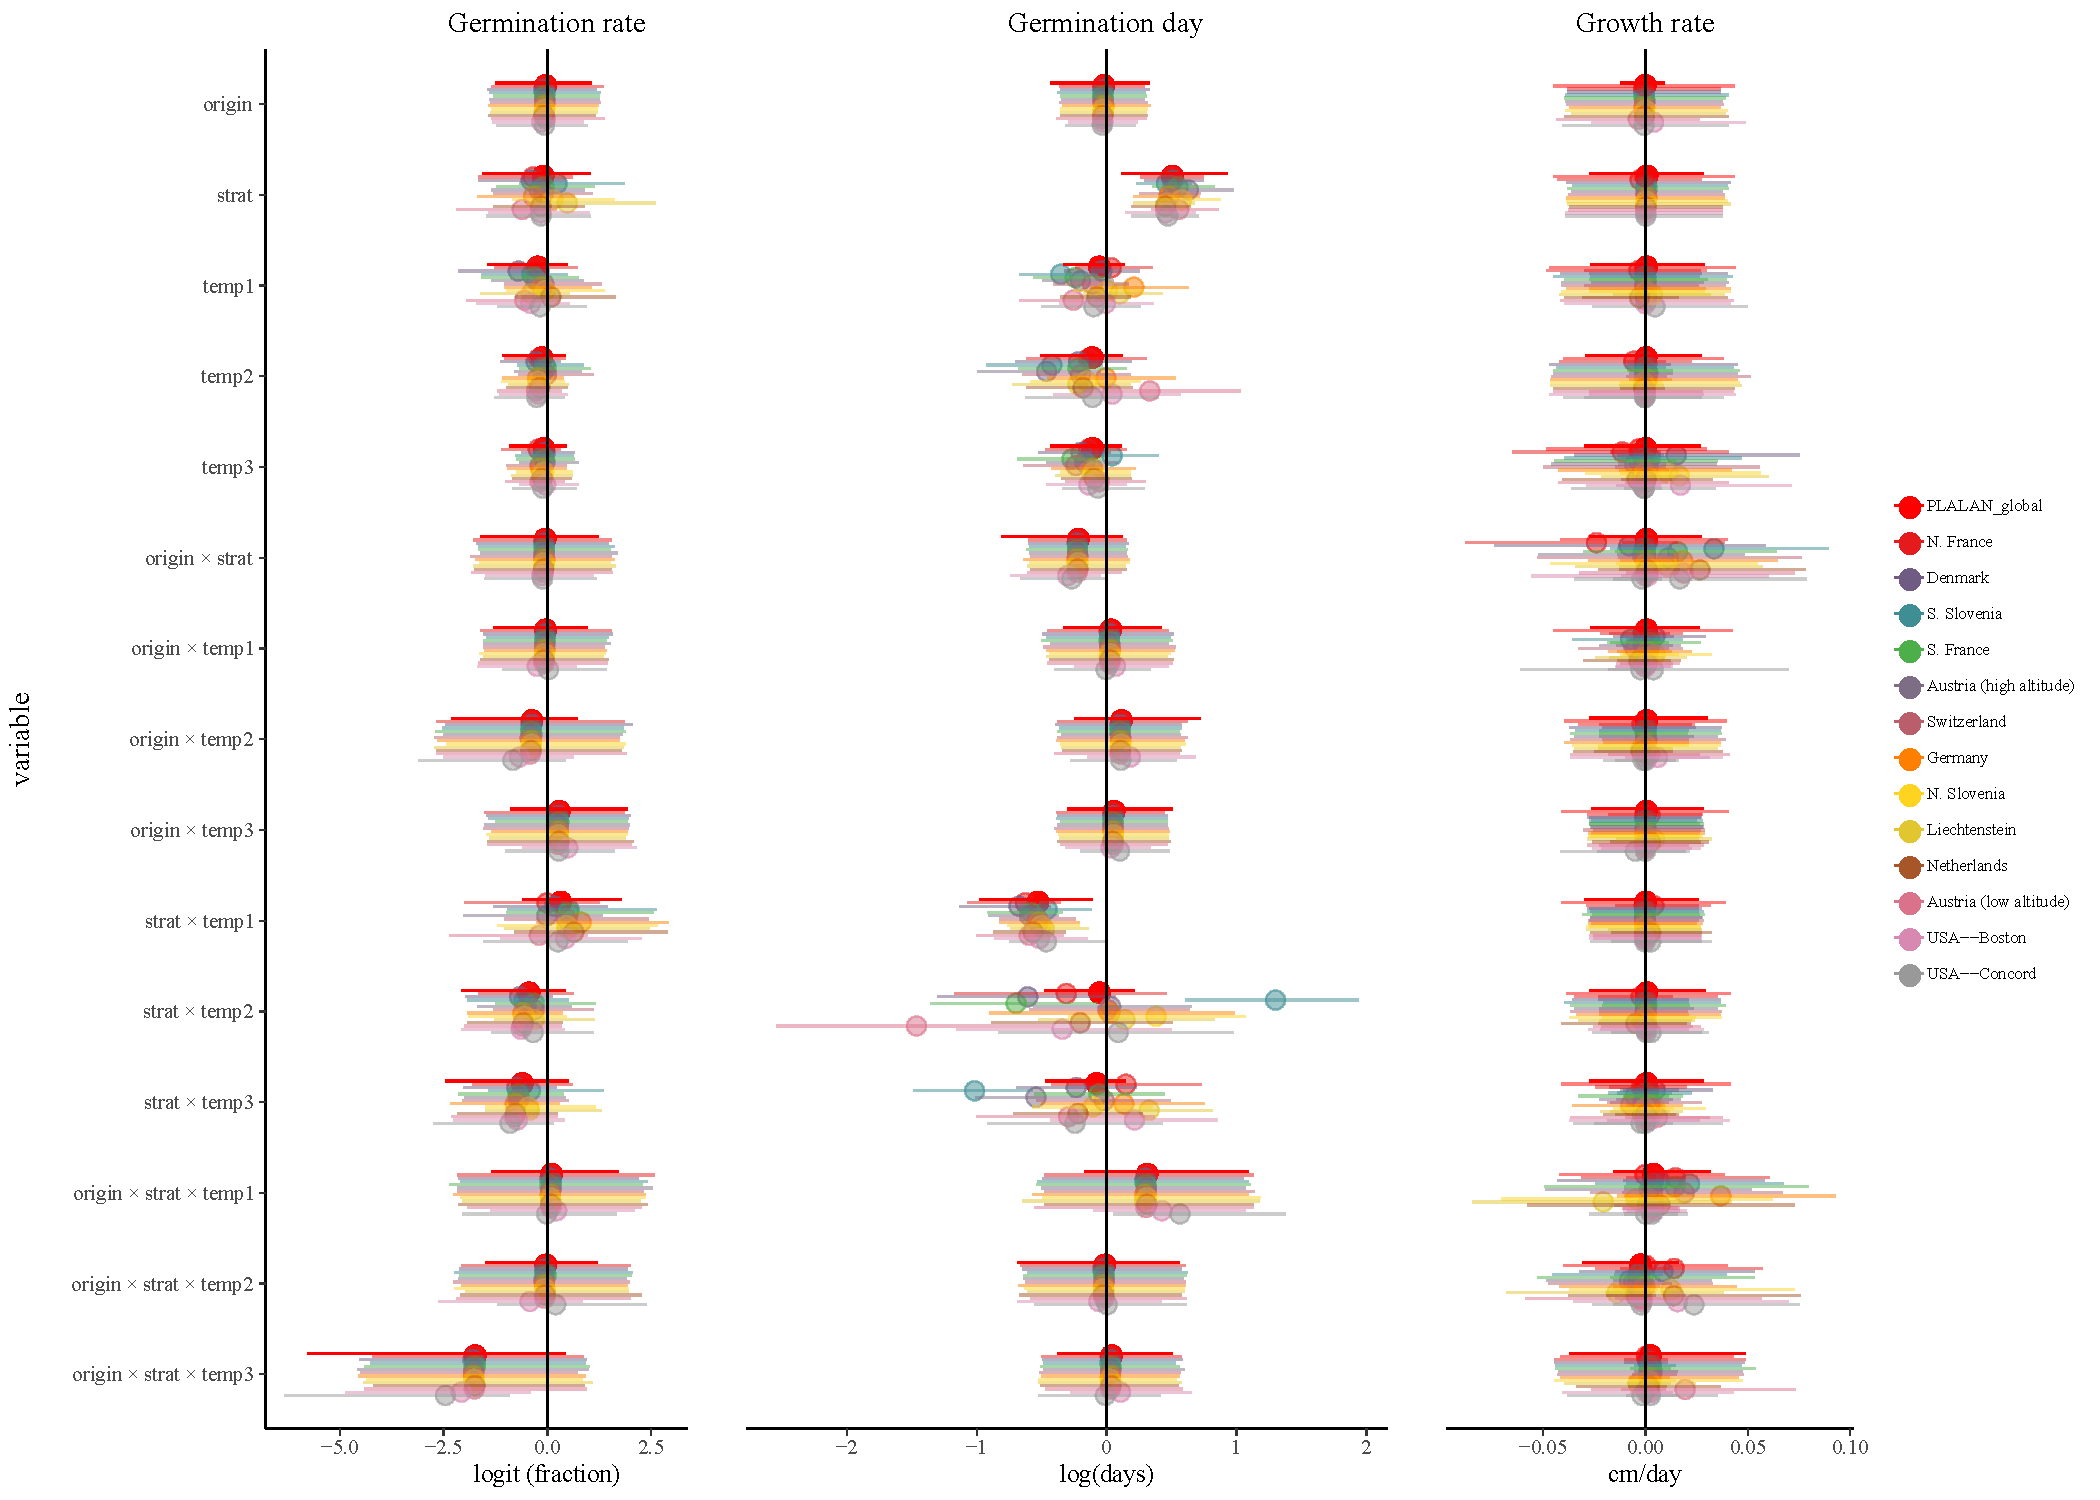
\includegraphics[scale=.7]{PLALAN_pops_plot.pdf}
\caption{Germination success, germination timing, and growth rate multilevel model coefficients with 95\% credible intervals for \textit{Plantago lanceolata}, showing main random effect for the species and random effects of each population. Zero represents the global mean fixed effect across all species. All values are relative to the intercept coefficients (see Tables \ref{tab:mod_rate_intercept}, \ref{tab:mod_time_intercept}, \ref{tab:mod_gr_intercept}). The reference level for temperature is a high of 18$^\circ$C, sixty days is the reference level for stratification (strat), and Europe is the reference level for origin.  Parameters testing for effects only of stratification or temperature are in black, while parameter testing for rapid evolution vs. broad environmental tolerance (i.e., those parameters containing ‘origin') are in red.}
\label{fig:pops}
\end{figure}
\clearpage
}



% latex table generated in R 4.0.3 by xtable 1.8-4 package
% Thu Apr 22 23:23:11 2021
\begin{longtable}{rrrrrrr}
\caption{Germination success model intercepts across all species (global intercept), across all populations of PLALAN (PLALAN intercept), and for each population of PLALAN. Note that all PLALAN intercepts are relative to the global intercept.  Output is in logit(fraction germinated)} \\ 
  & mean & sd & 2.5\% & 50\% & 97.5\% & Rhat \\ 
  \hline
global intercept & 1.85 & 0.64 & 0.65 & 1.82 & 3.26 & 1.00 \\ 
  PLALAN intercept & -0.33 & 0.63 & -1.82 & -0.21 & 0.76 & 1.00 \\ 
  N. France PLALAN intercept & -1.54 & 0.75 & -3.08 & -1.52 & -0.15 & 1.00 \\ 
  Denmark PLALAN intercept & -1.25 & 0.70 & -2.68 & -1.24 & 0.09 & 1.00 \\ 
  S. Slovenia PLALAN intercept & 1.55 & 0.79 & 0.09 & 1.51 & 3.20 & 1.00 \\ 
  S. France PLALAN intercept & 1.03 & 0.81 & -0.56 & 1.01 & 2.68 & 1.00 \\ 
  Austria (high altitude) PLALAN intercept & 0.77 & 0.77 & -0.71 & 0.76 & 2.29 & 1.00 \\ 
  Switzerland PLALAN intercept & 1.13 & 0.83 & -0.43 & 1.10 & 2.87 & 1.00 \\ 
  Germany PLALAN intercept & -2.10 & 0.82 & -3.75 & -2.07 & -0.56 & 1.00 \\ 
  N. Slovenia PLALAN intercept & 0.87 & 0.79 & -0.63 & 0.86 & 2.52 & 1.00 \\ 
  Liechtenstein PLALAN intercept & 0.70 & 0.78 & -0.77 & 0.69 & 2.27 & 1.00 \\ 
  The Netherlands PLALAN intercept & -0.03 & 0.73 & -1.45 & -0.03 & 1.36 & 1.00 \\ 
  Austria (low altitude) PLALAN intercept & -1.82 & 0.77 & -3.40 & -1.82 & -0.35 & 1.00 \\ 
  USA--Boston PLALAN intercept & -0.31 & 0.91 & -2.09 & -0.31 & 1.47 & 1.00 \\ 
  USA--Concord PLALAN intercept & -0.18 & 0.98 & -2.09 & -0.17 & 1.74 & 1.00 \\ 
  \hline
\label{tab:mod_rate_intercept}
\end{longtable}




% latex table generated in R 4.0.3 by xtable 1.8-4 package
% Thu Apr 22 23:23:11 2021
\begin{longtable}{rrrrrrr}
\caption{Germination timing model intercepts across all species (global intercept), across all populations of PLALAN (PLALAN intercept), and for each population of PLALAN. Note that all PLALAN intercepts are relative to the global intercept.  Output is in log(days to germination)} \\ 
  & mean & sd & 2.5\% & 50\% & 97.5\% & Rhat \\ 
  \hline
global intercept & 2.66 & 0.28 & 2.11 & 2.67 & 3.20 & 1.00 \\ 
  PLALAN intercept & 0.41 & 0.29 & -0.16 & 0.40 & 0.98 & 1.00 \\ 
  N. France PLALAN intercept & -0.03 & 0.12 & -0.29 & -0.02 & 0.22 & 1.00 \\ 
  Denmark PLALAN intercept & 0.09 & 0.12 & -0.11 & 0.07 & 0.37 & 1.00 \\ 
  S. Slovenia PLALAN intercept & 0.02 & 0.11 & -0.19 & 0.01 & 0.25 & 1.00 \\ 
  S. France PLALAN intercept & 0.03 & 0.11 & -0.19 & 0.02 & 0.26 & 1.00 \\ 
  Austria (high altitude) PLALAN intercept & 0.22 & 0.16 & -0.02 & 0.20 & 0.56 & 1.01 \\ 
  Switzerland PLALAN intercept & -0.06 & 0.12 & -0.32 & -0.05 & 0.15 & 1.00 \\ 
  Germany PLALAN intercept & 0.04 & 0.13 & -0.19 & 0.03 & 0.32 & 1.00 \\ 
  N. Slovenia PLALAN intercept & -0.04 & 0.11 & -0.27 & -0.02 & 0.17 & 1.00 \\ 
  Liechtenstein PLALAN intercept & -0.15 & 0.14 & -0.45 & -0.13 & 0.06 & 1.00 \\ 
  The Netherlands PLALAN intercept & -0.02 & 0.11 & -0.26 & -0.02 & 0.20 & 1.00 \\ 
  Austria (low altitude) PLALAN intercept & 0.03 & 0.12 & -0.20 & 0.02 & 0.30 & 1.00 \\ 
  USA--Boston PLALAN intercept & -0.06 & 0.14 & -0.38 & -0.04 & 0.20 & 1.00 \\ 
  USA--Concord PLALAN intercept & -0.04 & 0.14 & -0.35 & -0.02 & 0.23 & 1.00 \\ 
  \hline
\label{tab:mod_time_intercept}
\end{longtable}




% latex table generated in R 4.0.3 by xtable 1.8-4 package
% Thu Apr 22 23:23:11 2021
\begin{longtable}{rrrrrrr}
\caption{Growth rate model intercepts across all species (global intercept), across all populations of PLALAN (PLALAN intercept), and for each population of PLALAN. Note that all PLALAN intercepts are relative to the global intercept.  Output is in cm/dat} \\ 
  & mean & sd & 2.5\% & 50\% & 97.5\% & Rhat \\ 
  \hline
global intercept & 0.17 & 0.05 & 0.08 & 0.17 & 0.27 & 1.00 \\ 
  PLALAN intercept & -0.03 & 0.05 & -0.12 & -0.03 & 0.07 & 1.00 \\ 
  N. France PLALAN intercept & -0.01 & 0.01 & -0.03 & -0.01 & 0.02 & 1.00 \\ 
  Denmark PLALAN intercept & -0.03 & 0.01 & -0.05 & -0.03 & -0.01 & 1.00 \\ 
  S. Slovenia PLALAN intercept & 0.01 & 0.01 & -0.01 & 0.01 & 0.03 & 1.00 \\ 
  S. France PLALAN intercept & 0.00 & 0.01 & -0.02 & 0.00 & 0.02 & 1.00 \\ 
  Austria (high altitude) PLALAN intercept & -0.00 & 0.01 & -0.03 & -0.00 & 0.02 & 1.00 \\ 
  Switzerland PLALAN intercept & -0.00 & 0.01 & -0.02 & -0.00 & 0.02 & 1.00 \\ 
  Germany PLALAN intercept & 0.01 & 0.01 & -0.01 & 0.01 & 0.04 & 1.00 \\ 
  N. Slovenia PLALAN intercept & 0.02 & 0.01 & -0.00 & 0.02 & 0.04 & 1.00 \\ 
  Liechtenstein PLALAN intercept & 0.01 & 0.01 & -0.01 & 0.01 & 0.03 & 1.00 \\ 
  The Netherlands PLALAN intercept & 0.01 & 0.01 & -0.02 & 0.01 & 0.03 & 1.00 \\ 
  Austria (low altitude) PLALAN intercept & -0.02 & 0.01 & -0.05 & -0.02 & 0.00 & 1.00 \\ 
  USA--Boston PLALAN intercept & 0.00 & 0.01 & -0.03 & 0.00 & 0.03 & 1.00 \\ 
  USA--Concord PLALAN intercept & -0.01 & 0.02 & -0.04 & -0.01 & 0.02 & 1.00 \\ 
  \hline
\label{tab:mod_gr_intercept}
\end{longtable}


\end{document}
